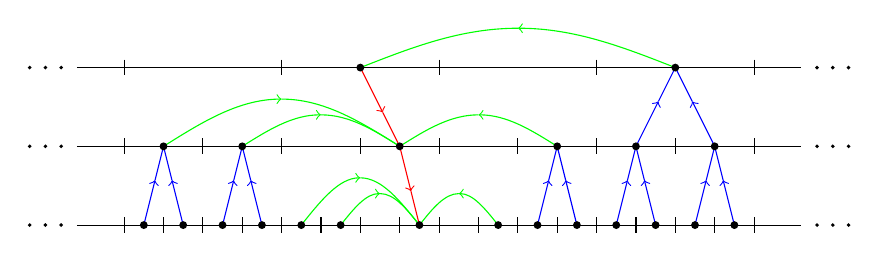
\begin{tikzpicture}[scale = 2.0]
  \def \cdotssizes{0.0125};
  \def \cdotspacing{0.1};
  \def \nodesize{0.025};
  \def \leftextent{0};
  \def \rightextent{4};
  \def \hmargin{0.3};
  \def \hrulertickheight{0.1};
  \def \yone {0.0};
  \def \ytwo {0.5};
  \def \ythree {1.0};
  \def \yfour {1.5};

  % Draw horizontal rulers and cdots on the sides.
  \foreach \y in {\yone, \ytwo, \ythree} {
    \draw [-] ({\leftextent - \hmargin}, \y) -- ({\rightextent + \hmargin}, \y);
    \foreach \i in {1, 2, 3} {
      \fill[black] ({\leftextent - \hmargin - (\i * \cdotspacing)}, \y) circle (\cdotssizes);
      \fill[black] ({\rightextent + \hmargin + (\i * \cdotspacing)}, \y) circle (\cdotssizes);
    }
  };
  
  % Draw ticks on each horizontal ruler.
  \foreach \x in {\leftextent, 1.0, ..., \rightextent} {
    \draw [-] (\x, {\ythree + (\hrulertickheight / 2)}) -- (\x, {\ythree - (\hrulertickheight / 2)});
  };
  \foreach \x in {\leftextent, 0.5, ..., \rightextent} {
    \draw [-] (\x, {\ytwo + (\hrulertickheight / 2)}) -- (\x, {\ytwo - (\hrulertickheight / 2)});
  };
  \foreach \x in {\leftextent, 0.25, ..., \rightextent} {
    \draw [-] (\x, {\yone + (\hrulertickheight / 2)}) -- (\x, {\yone - (\hrulertickheight / 2)});
  };
  
  % Draw SS translation arrows.
  \def \theta {4/7}
  \foreach \x in {0.25, 0.75, 2.75, 3.25, 3.75} {
    \def \midpt {(1 - \theta) * \yone + \theta * \ytwo};
    \draw [-, blue] (\x, \ytwo) -- ({\x - 0.125*(1 - \theta)}, {\midpt});
    \draw [<-, blue] ({\x - 0.125*(1 - \theta)}, {\midpt}) -- ({\x - 0.125}, \yone);
    \draw [-, blue] (\x, \ytwo) -- ({\x + 0.125*(1 - \theta)}, {\midpt});
    \draw [<-, blue] ({\x + 0.125*(1 - \theta)}, {\midpt}) -- ({\x + 0.125}, \yone);
  };
  \foreach \x in {3.5} {
    \def \midpt {(1 - \theta) * \ytwo + \theta * \ythree};
    \draw [-, blue] (\x, \ythree) -- ({\x - 0.25*(1 - \theta)}, {\midpt});
    \draw [<-, blue] ({\x - 0.25*(1 - \theta)}, {\midpt}) -- ({\x - 0.25}, \ytwo);
    \draw [-, blue] (\x, \ythree) -- ({\x + 0.25*(1 - \theta)}, {\midpt});
    \draw [<-, blue] ({\x + 0.25*(1 - \theta)}, {\midpt}) -- ({\x + 0.25}, \ytwo);
  };
  
  % Draw RR translation arrows.
  \def \theta {3/7}
  \foreach \x in {1.75} {
    \def \midpt {(1 - \theta) * \yone + \theta * \ytwo};
    \draw [->, red] (\x, \ytwo) -- ({\x + 0.125*(1 - \theta)}, {\midpt});
    \draw [-, red] ({\x + 0.125*(1 - \theta)}, {\midpt}) -- ({\x + 0.125}, \yone);
  };
  \foreach \x in {1.5} {
    \def \midpt {(1 - \theta) * \ytwo + \theta * \ythree};
    \draw [->, red] (\x, \ythree) -- ({\x + 0.25*(1 - \theta)}, {\midpt});
    \draw [-, red] ({\x + 0.25*(1 - \theta)}, {\midpt}) -- ({\x + 0.25}, \ytwo);
  };

  % Draw SR translation arrows.
  \def \center {1.5}
  \foreach \x in {3.5} {
    \pgfmathsetmacro{\xmid}{(\center + \x)/2};
    \pgfmathsetmacro{\ymid}{(\ythree + \yfour)/2};
    \draw[->, green] (\x, \ythree) sin (\xmid, \ymid);
    \draw[-, green] (\xmid, \ymid) cos (\center, \ythree);
  };
  \def \center {1.75}
  \pgfmathsetmacro{\maxdist}{abs(\center - 0.25)};
  \foreach \x in {0.25, 0.75, 2.75} {
    \pgfmathsetmacro{\dist}{abs(\center - \x)};
    \pgfmathsetmacro{\theta}{0.6 * \dist / abs(\maxdist)};
    \pgfmathsetmacro{\xmid}{(\center + \x)/2};
    \pgfmathsetmacro{\ymid}{(1 - \theta) * \ytwo + \theta * \ythree};
    \draw[->, green] (\x, \ytwo) sin (\xmid, \ymid);
    \draw[-, green] (\xmid, \ymid) cos (\center, \ytwo);
  };
  \def \center {1.875}
  \pgfmathsetmacro{\maxdist}{abs(\center - 1.125)};
  \foreach \x in {1.125, 1.375, 2.375} {
    \pgfmathsetmacro{\dist}{abs(\center - \x)};
    \pgfmathsetmacro{\theta}{0.6 * \dist / abs(\maxdist)};
    \pgfmathsetmacro{\xmid}{(\center + \x)/2};
    \pgfmathsetmacro{\ymid}{(1 - \theta) * \yone + \theta * \ytwo};
    \draw[->, green] (\x, \yone) sin (\xmid, \ymid);
    \draw[-, green] (\xmid, \ymid) cos (\center, \yone);
  };
  
  % Draw node circles.
  \foreach \x in {1.5, 3.5} {
    \fill[black] (\x, \ythree) circle (\nodesize);
  };
  \foreach \x in {0.25, 0.75, 1.75, 2.75, 3.25, 3.75} {
    \fill[black] (\x, \ytwo) circle (\nodesize);
  };
  \foreach \x in {0.125, 0.375, 0.625, 0.875, 1.125, 1.375, 1.875, 2.375, 2.625, 2.875, 3.125, 3.375, 3.625, 3.875} {
    \fill [black] (\x, \yone) circle (\nodesize);
  };
\end{tikzpicture} \\

%%% Local Variables:
%%% mode: latex
%%% TeX-master: "../paper/paper"
%%% End:
